\chapter {Analýza}

\section {Magnetická rezonancia}

Magnetická rezonancia (MR) je jedna zo zobrazovacích techník, ktorá je používaná k zobrazeniu vnútorných orgánov tela.
Narozdiel od röntgenového žiarenia a počítačovej tomografie (CT), magnetická rezonancia nepoužíva ionizujúce žiarenie. Avšak medzi spoločné znaky týchto troch zobrazovacích techník patrí ich neinvazívnosť a bezbolestné vyšetrenie \cite{basic_principles_of_mri} (vlastný preklad). \newline

Magnetická rezonancia sa používa najmä pri:
\begin {itemize}
\item {podozrení na anomálie mozgu a miechy, nádory a cysty,}
\item {poranení kĺbov a mäkkých tkanív,}
\item {podozrení na srdcové problémy,}
\item {rozličných ochoreniach pečene a iných brušných orgánov, atď. \cite{mr_usage} (vlastný preklad).}
\end {itemize}

Pred niektorými MR procedúrami sa pacientovi intravenózne môže podať kontrastná látka, ktorá zlepší kontrast a vzájomnú odlíšiteľnosť orgánov a mäkkých tkanív \cite{contrast_agents}.

Bohužiaľ, existujú aj určité kontraindikácie, pri ktorých použitie MR pre daného človeka nie je možné.
Jedným z kontraindikácií je implantovaný kardiostimulátor, v prípade že nie je kompatibilný s MR. Všeobecne je kontraindikácia použitie akéhokoľvek magnetického materiálu v tele. Taktiež je MR vyšetrenie kontraindikované ženám v prvom trimestri tehotenstva \cite{mr_contraindications}.

\subsection {Princíp magnetickej rezonancie}

Princípom magnetickej rezonancie je smerové magnetické pole (moment - $\mathcal{B}_{0}$) spojené s pohybom voľných jadier vodíku v tele subjektu. Tieto jadrá majú charakteristický pohyb (spin) vytvárajúci malý magnetický moment s určitým smerom (ktorý je náhodný) a veľkosťou. Keď je subjekt umiestnený vo veľkom magnetickom poli (v tubuse MR prístroja), voľné vodíkové jadrá sa zarovnajú v smere $\mathcal{B}_{0}$ (smer $y$) a vytvoria magnetický moment $\mathcal{M}$ paralelne k $\mathcal{B}_{0}$. Vodíkové jadrá začnú náhle prechádzať okolo smeru magnetického poľa ako gyroskopy -- toto správanie sa nazýva Larmorova precesia \cite{basic_principles_of_mri} (vlastný preklad).

\begin {center}
        \centering
        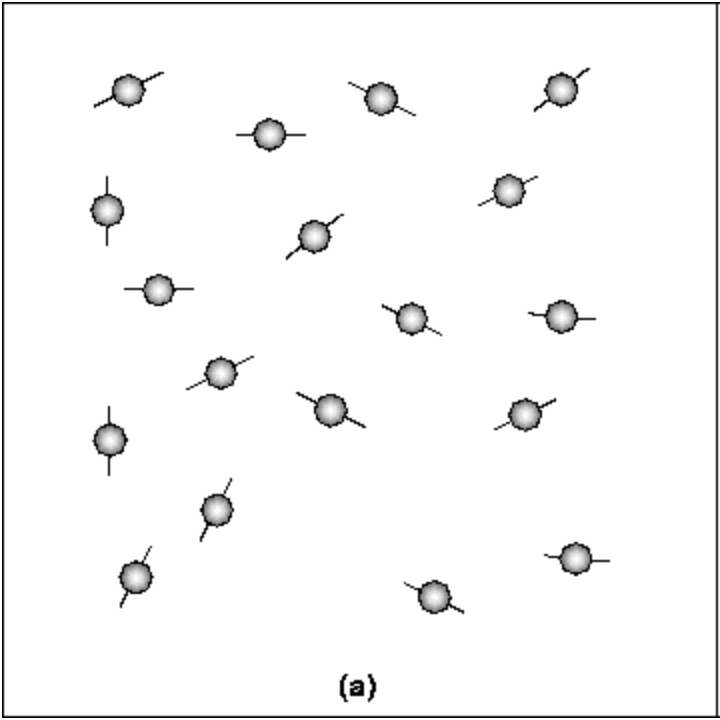
\includegraphics[width=6cm, height=6cm]{media/hydrogen_moving_freely.png}
        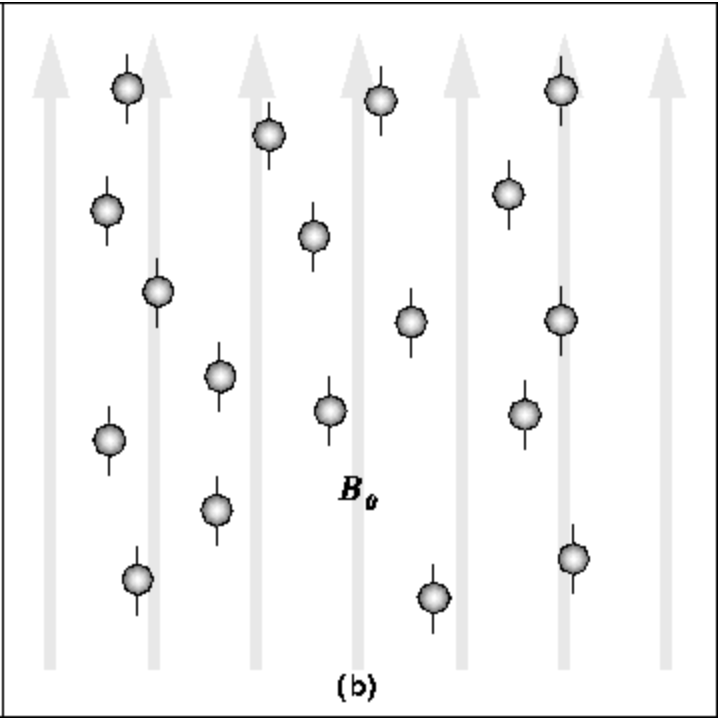
\includegraphics[width=6cm, height=6cm]{media/hydrogen_oscilating.png}
        \captionof{figure}[Voľný pohyb vodíkových jadier a ich zarovnanie v smere $\mathcal{B}_{0}$]{Na ľavom obrázku je možné vidieť voľný pohyb vodíkových jadier a na pravom ich zarovnanie v smere $\mathcal{B}_{0}$ \cite{basic_principles_of_mri}.}
\end {center}

Následne sa aplikuje rádiofrekvenčný impulz $\mathcal{B}_{rf}$ kolmo na $\mathcal{B}_{0}$.
Tento impulz rovnajúci sa frekvencii Larmorovej precesie spôsobí posun $\mathcal{M}$ od $\mathcal{B}_{0}$ \cite{basic_principles_of_mri} (vlastný preklad).

\begin {center}
        \centering
        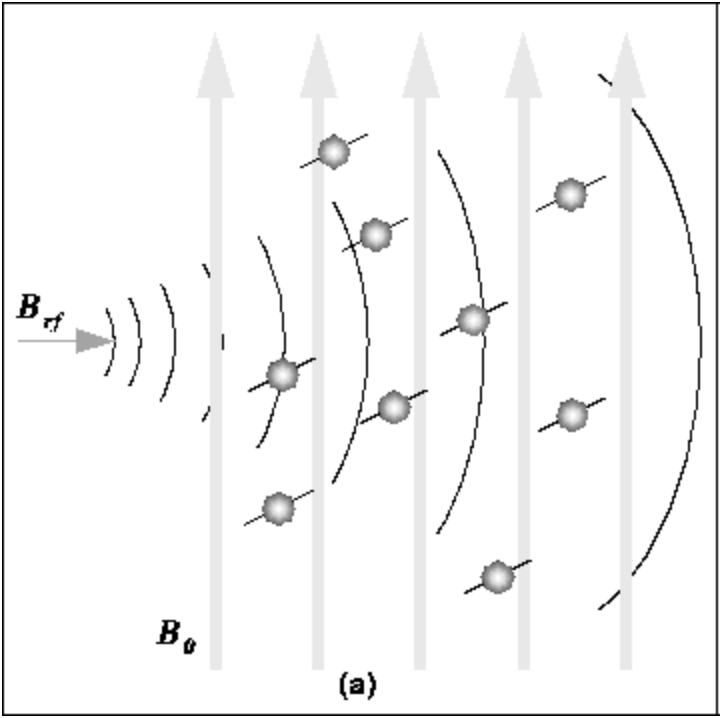
\includegraphics[width=6cm, height=6cm]{media/hydrogen_reacting_to_rf.png}
        \captionof{figure}[Kolmá aplikácia RF impulzu $\mathcal{B}_{rf}$ na vodíkové jadrá]{Kolmá aplikácia RF impulzu $\mathcal{B}_{rf}$ na vodíkové jadrá \cite{basic_principles_of_mri}.}
\end {center}

Frekvenciu Larmorovej precesie (nazývaná ako Larmorova frekvencia), je definovaná nasledovne:

\begin {center}
$\omega_{0}$ = $-\gamma * \mathcal{B}_{0}$,
\end {center}

kde $\gamma$ predstavuje gyromagnetický pomer a $\mathcal{B}_{0}$ intenzitu magnetického poľa.
Gyromagnetický pomer je špecifická konštanta závislá na jadre danej častice. Pre vodík sa táto konštanta rovná 42.6 MHz/Tesla \cite{basic_principles_of_mri} (vlastný preklad). \newline

Akonáhle prestane pôsobiť rádiofrekvenčný impulz $\mathcal{B}_{rf}$, jadrá vodíka sa presunú naspäť tak, že ich $\mathcal{M}$ je znovu paralelný s $\mathcal{B}_{0}$. Tento návrat vodíkových jadier sa nazýva relaxácia. Počas nej jadrá strácajú energiu vysielaním ich vlastného rádiofrekvenčného signálu. Tento signál sa nazýva \uv{voľný indukčný rozpad} -- z anglického Free Induction Decay (FID). Tento signál sa zmeria vodivým poľom MR prístroja za účelom vyhotovenia 3D MR snímku v odtieňoch šedej \cite{basic_principles_of_mri} (vlastný preklad).

\begin {center}
        \centering
        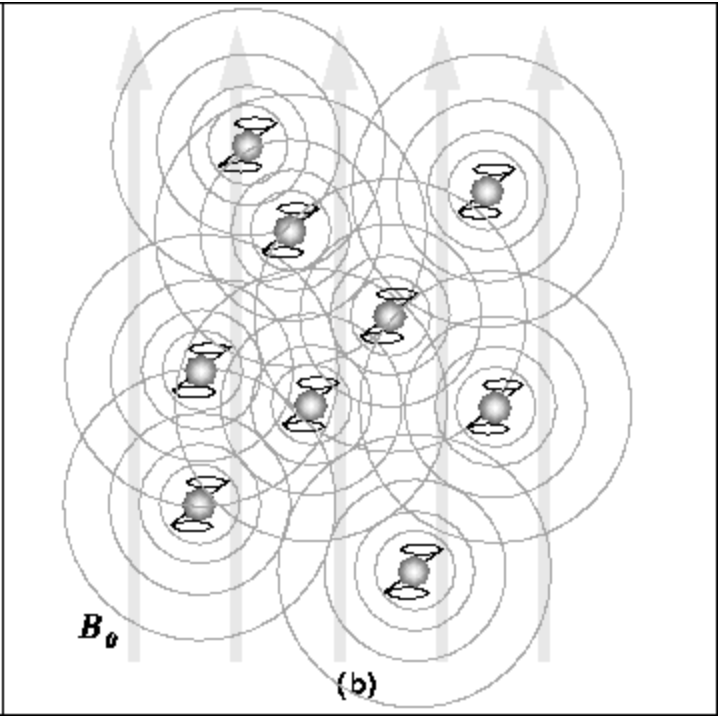
\includegraphics[width=6cm, height=6cm]{media/hydrogen_emitting_rf.png}
        \captionof{figure}[Emitovanie FID signálu vodíkovými jadrami]{Emitovanie FID signálu vodíkovými jadrami \cite{basic_principles_of_mri}.}
\end {center}

Avšak, na jeho vytvorenie musí byť FID signál enkódovaný pre každý rozmer pomocou frekvenčného a fázového kódovania. Kódovanie v axiálnom smere sa dosiahne pridaním gradientového magnetického poľa $\mathcal{G}_{y}$ v smere $\mathcal{B}_{0}$ (v smere $y$). Po pridaní $\mathcal{G}_{y}$ sa hodnota Larmorovej frekvencie zmení lineárne v axiálnom smere, tzn. že pre konkrétny axiálny rez existuje konkrétna Larmorova frekvencia, ktorá sa aplikuje vyslaním rádiofrekvenčného impulzu $\mathcal{B}_{rf}$. $\mathcal{G}_{y}$ sa potom odstráni a ďalší gradient, $\mathcal{G}_{x}$, sa aplikuje kolmo na $\mathcal{G}_{y}$. Výsledkom je, že rezonančné frekvencie jadier sa menia v smere $x$ vďaka $\mathcal{G}_{x}$ a majú fázovú variáciu v smere $y$ v dôsledku predtým aplikovaného $\mathcal{G}_{y}$. Vzorky v smere $x$ sú teda kódované frekvenciou a v smere $y$ fázou. 2D inverzná Fourierova transformácia sa následne použije na transformáciu vzoriek na snímku \cite{basic_principles_of_mri} (vlastný preklad). \newline

Kontrast získanej snímky závisí od nasledujúcich dvoch parametrov:

\begin {itemize}
\item {od času pozdĺžnej relaxácie - T1}
\item {a od času priečnej relaxácie - T2.}
\end {itemize}

Čas T1 je čas potrebný pre jadrá vodíkov k ich relaxácii a čas T2 predstavuje čas potrebný na to, aby sa FID signál prechádzajúci cez dané tkanivo rozpadol. Oba časy závisia od daného typu látky nachádzajúcej sa v subjekte \cite{basic_principles_of_mri} (vlastný preklad).

Po získaní MR snímky sa impulz $\mathcal{B}_{rf}$ opakuje vopred stanovenou rýchlosťou. Zmenou sekvencie impulzov ($\mathcal{B}_{rf}$) sa vytvárajú rôzne typy snímkov. Čas opakovania ($TR$) je množstvo času medzi po sebe nasledujúcimi pulznými sekvenciami aplikovanými na rovnaký rez. Time to Echo ($TE$) je čas medzi dodaním impulzu $\mathcal{B}_{rf}$ a prijatím odozvy. Úpravou $TR$ je možné meniť výsledný kontrast na snímke medzi rôznymi typmi tkanív \cite{basic_principles_of_mri} (vlastný preklad). \clearpage

\section {SPAMM}

SPAMM -- z anglického (SPAtial Modulation of Magnetization) $\rightarrow$ \uv{priestorová modulácia magnetizácie} -- je technika, ktorá používa rádiofrekvenčné saturačné impulzy pre umiestnenie mriežky na myokard, za cieľom sledovania jej pohybu počas srdcového cyklu.

V súčasnej praxi sa SPAMM technika používa v situáciách, kde informácia o kontrakcii myokardu je kľúčová, ako napr. podozrenie na ischemickú chorobu srdca alebo abnormality týkajúcej sa neprirodzeného pohybu steny myokardu \cite{spamm_description} (vlastný preklad).

\begin {center}
        \centering
        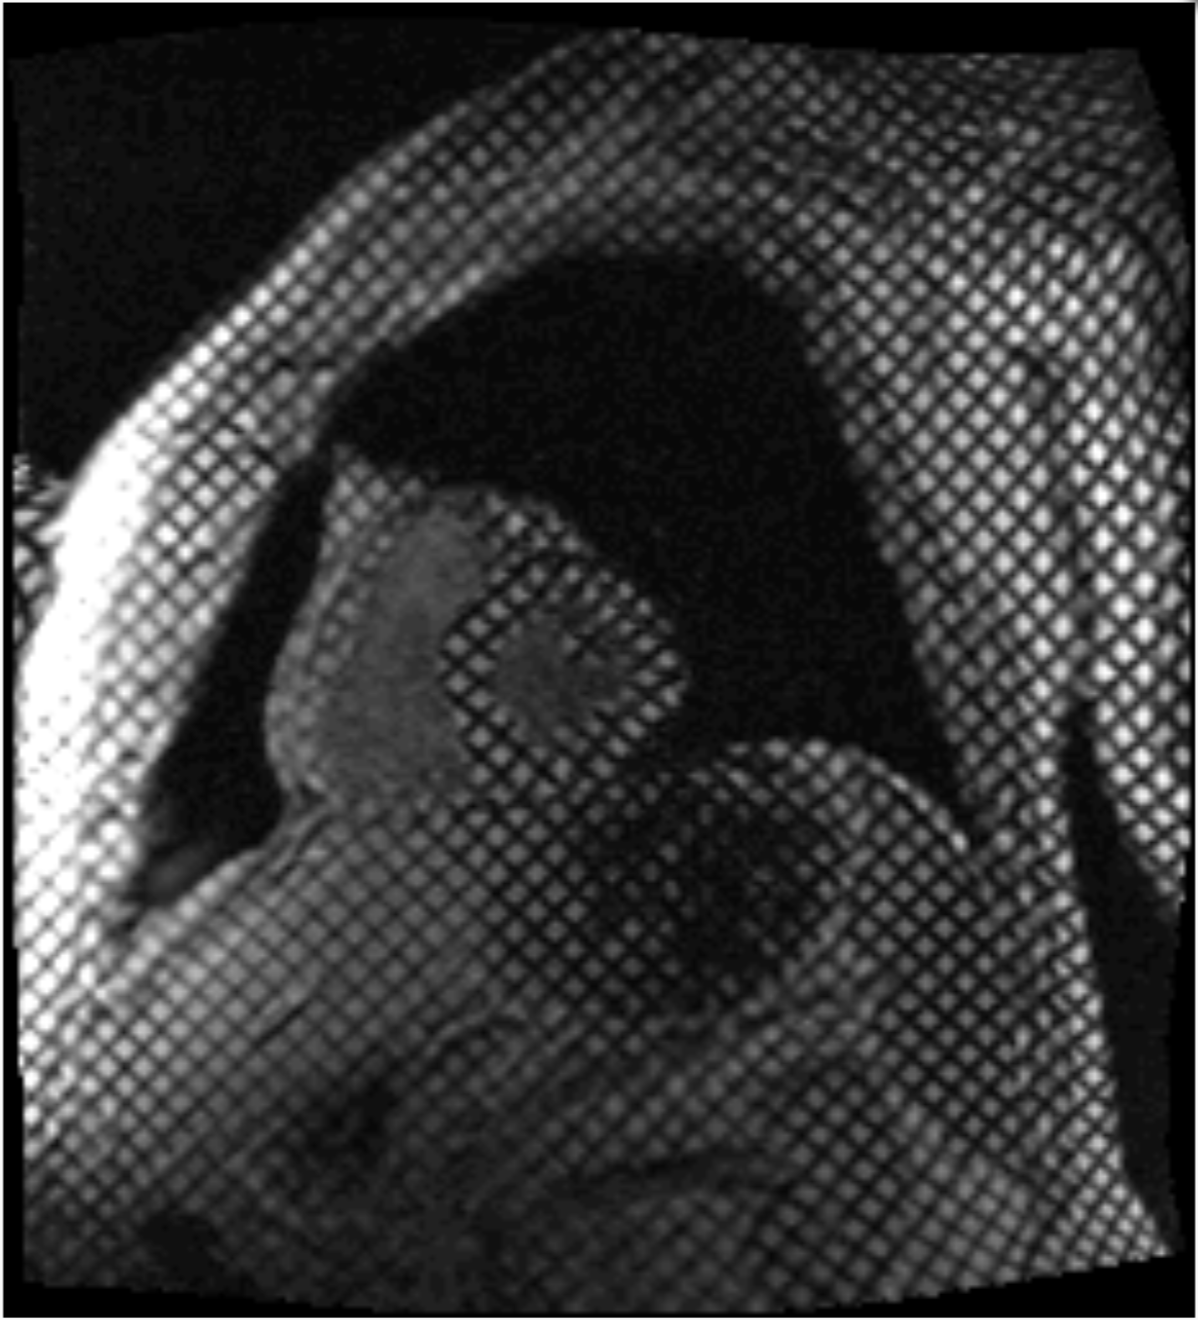
\includegraphics[width=6cm, height=6cm]{media/tagged_heart.png}
        \captionof{figure}[Tagovaný snímok myokardu pomocou techniky SPAMM]{Otagovaný snímok myokardu pomocou techniky SPAMM \cite{spamm_description}.}
\end {center}

Nevýhodou použitia tejto techniky je skutočnosť, že táto mriežka sa stráca s blížiacim sa koncom srdcového cyklu. Samotné čiary mriežky sa pri konci systoly (časť srdcového cyklu, počas ktorej sa komory srdca sťahujú po naplnení krvou) môžu zlúčiť alebo úplne vyblednúť, čo sťažuje následnú analýzu pohybu srdca \cite{spamm_description} (vlastný preklad).

\begin {center}
        \centering
        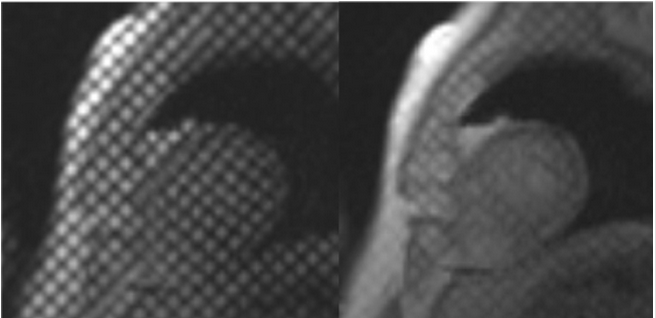
\includegraphics[width=10cm, height=5cm]{media/early_late_systole.png}
        \captionof{figure}[Ukážka vyblednutia SPAMM mriežky]{Ľavý obrázok zobrazuje začiatok systoly, pravý jej koniec.}
\end {center}

\pagebreak

\section {Analýza súčasnej aplikácie}

V tejto sekcii sa budem zaoberať analýzou súčasnej aplikácie, ktorá zahŕňa popis jej funkcionality spolu s vizualizáciami...

\subsection {Popis aplikácie}

Cameo je desktopová aplikácia schopná zobrazovať sériu snímkov myokardu, ktoré pochádzajú z MR. Taktiež zobrazuje doplňujúce údaje, ako napr. údaje o pacientovi, detaily o zobrazených snímkoch a detaily série týchto snímkov. Okrem samotného zobrazenia myokardu aplikácia umožňuje tiež analyzovať myokard. V našom prípade sa analýza myokardu týka jeho pohybu.

Pre analýzu srdcového svalu je potrebné najprv do aplikácie nahrať sériu snímkov, ktoré sú otagované priestorovou moduláciou magnetizácie popísanou vyššie. Táto mriežka sa na každom snímku deformuje podľa pohybu tkaniva. Na počiatočných snímkoch je mriežka dobre viditeľná, avšak jej viditeľnosť sa každým ďalším snímkom zmenšuje. Tento efekt je spôsobený poklesom Nevýhodou  Pohyb myokardu je možný analyzovať vďaka 


Túto aplikáciu môžeme rozdeliť na x častí - potom popíšem každú časť.

\subsection {Použité technológie}

\subsubsection {DICOM}\label{dicom}

V súčasnosti sú snímky získané pomocou zobrazovacích techník v medicíne zväčša ukladané v archivačnom a komunikačnom systéme snímkov. Tento systém ukladá nielen snímkové dáta ale aj iné relevantné dáta k týmto snímkam podľa štandardu známom ako DICOM (Digital Imaging and Communications in Medicine) \cite{Varma_2012} (vlastný preklad). Ten je medzinárodným štandardom pre komunikáciu a manažment informácií o medicínskych obrazových a k nim príslušných dátach. Definuje, ako majú byť takéto dáta spracovávané, ukladané, tlačené a prenášané medzi zariadeniami podporujúcimi príjem týchto dát \cite{about_dicomlibrary} (vlastný preklad).

DICOM štandard bol vyvíjaný na prelome 80. a 90. rokoch 20. storočia v spolupráci medzi American College of Radiology a National Electrical Manufacturers Association \cite{dicom_history} (vlastný preklad). Momentálne sa skladá z 22 nezávislých častí, z ktorých avšak nie všetky musia byť implementované daným zariadením podporujúcim tento štandard.

Pre účely spracovania snímkových dát, DICOM štandard vo svojej 10. časti definuje dátovú štruktúru (formát) súboru, do ktorého sa tieto dáta ukladajú. Dátová štruktúra súboru, ktorý spĺňa podmienky 10. časti tohto štandaru, býva značená ako \uv{DICOM Part 10} súbor, inak známy ako DICOM súbor \cite{Varma_2012} (vlastný preklad).

Štruktúra tohto (binárneho) súboru je nasledovná -- prvých 128 bajtov býva zväčša prázdnych (vyplnených 0). Ďalšie 4 bajty obsahujú uložený reťazec \uv{DICM}.  Na základe týchto bajtov sa dá určiť, či sa jedná alebo nejedná o DICOM súbor.
Ďalej nasleduje hlavička, ktorá je rozdelená na viacero skupín zoskupujúcich súvisiace atribúty. Konkrétne atribúty sa adresujú tagom - ten sa skladá z 8 čísiel v hexadecimálnom formáte. Prvé 4 čísla reprezentujú skupinu, v ktorej sa daný atribút nachádza a posledné 4 čísla jednoznačne identifikujú konkrétny atribút v skupine \cite{Varma_2012} (vlastný preklad).

Ako príklad bude uvedené získanie informácie o pacientovom veku - všetky informácie o pacientovi sa nachádzajú v skupine 0010. Pacientov vek v tejto skupine sa nachádza na pozícii 1010, tým pádom výsledný tag pod ktorým nájdeme vek pacienta je (0010, 1010). Ku každému tagu je jednoznačne priradená reprezentácia jej hodnoty (VR), ktorý určuje dátový typ, formát a dĺžku hodnoty daného atribútu  \cite{Varma_2012} (vlastný preklad).

Po hlavičke nasleduje skupina 7FE0, ktorá už obsahuje dáta o samotných obrazových pixeloch \cite{Varma_2012} (vlastný preklad). Typ kódovania týchto dát určuje Transfer Syntax -- ten udáva, akým spôsobom sú obrazové pixely zakódované. Transfer Syntax obsahuje taktiež informáciu, v akom poradí bajtov sú informácie zakódované (Little Endian vs Big Endian) a aká kompresia obrazových dát bola použitá \cite{dicom_transfer_syntax} (vlastný preklad).

\subsubsection {Qt}

\quad Súčasná aplikácia bola vyvinutá pomocou Qt -- cross-platformového frameworku určeného pre vytváranie aplikácií najmä v jazyku C\texttt{++}. Aplikácie vyvinuté týmto frameworkom majú výhodu v tom, že sú spustiteľné na rôznych operačných systémoch s minimálnym počtom zmien v zdrojovom kóde \cite{qt_description} (vlastný preklad).

Výsadou tohto frameworku je taktiež rozdelenie jeho funkcionality do jednotlivých modulov. Pri následom vytváraní aplikácie sa použijú len také moduly, ktoré sú v danej aplikácii potrebné \cite{qt_description} (vlastný preklad).

V súčasnej aplikácii boli použité nasledovné moduly: 

\begin{itemize}
\item {Qt Core}
\item {Qt Widgets}
\item {Qt GUI}
\item {Qt Test}
\end{itemize}

Qt Core modul obsahuje najpoužívanejšie triedy ako napr. \lstinline{QCoreApplication}, \lstinline{QObject}, \lstinline{QDebug} a iné. Nakoľko sú tieto triedy používané aj inými modulmi, je tento modul implicitne nalinkovaný Qt frameworkom pri budovaní aplikácie \cite{qtcore_description} (vlastný preklad). \newline

Qt Widgets modul poskytuje UI elementy, ktoré sú určené pre vytváranie používateľského rozhrania. Tieto elementy môžu zobrazovať rozličné dáta, prijímať vstup z klávesnice, byť štylizované a zoskupované do rozličných usporiadaní \cite{qtwidgets_description} (vlastný preklad). Existujúca aplikácia používa z modulu napr. triedu \lstinline{QMainWindow}, ktorá je zodpovedná za vykreslenie aplikačného okna a taktiež triedu \lstinline{QGraphicsScene}, ktorá je zodpovedná za vykreslenie obrázkov z magnetickej rezonancie v DICOM formáte. \newline

Qt GUI modul obsahuje triedy určené pre zobrazovanie aplikačného okna a iného grafického obsahu s následnou obsluhou eventov udalostí. Taktiež obsahuje triedy, ktoré sú zodpovedné za zobrazovanie 2D grafiky, fontov a typografie \cite{qtgui_description} (vlastný preklad).
Súčasná aplikácia z tohto modulu používa napr. triedu \lstinline{QImage}, ktorá obsahuje metódy pre priamy prístup k pixelom obrázkov a ich manipuláciu. \newline

Qt Test modul je poskytuje rozličné triedy pre jednotkové testovanie Qt aplikácií a príslušných knižníc \cite{qttest_description} (vlastný preklad) -- v súčasnej aplikácii bol tento modul využitý pri testovaní grafického používateľského rozhrania a funkcionalít súčasnej aplikácie, ako napr. testovanie zmien v nastaveniach vykreslenej mriežky na obrázku z magnetickej rezonancie.

\subsubsection {Qmake}

Pre zjednodušenie písania Makefilov, ktoré definujú, ako má byť program skompilovaný, bol použitý nástroj Qmake. Ten umožňuje vývojárom definovať vytváranie rozličných Makefilov pre daný program pomocou syntaxu definovaného programom Qmake \cite{qmake_description} (vlastný preklad). Výsledkom tohto procesu je súbor s príponou \lstinline{.pro} obsahujúci inštrukcie, ako daný program skompilovať. Následne sa pomocou príkazu \lstinline{qmake} s argumentom cesty k \lstinline{.pro} súboru daný program skompiluje a jeho výsledkom je spustiteľný súbor aplikácie.

\subsubsection {DCMTK}

DCMTK je kolekcia knižníc a aplikácií, ktoré implementujú veľkú časť štandardu DICOM v jazykoch C a C\texttt{++}. Úlohou týchto knižníc je okrem iného skúmanie, vytváranie a konverzia DICOM súborov, manipulácia s pamäťovými médiami a odosielanie a prijímanie obrazových súborov cez internetové pripojenie. Používa sa v nemocniciach a rôznych spoločnostiach po celom svete, kde sa používa ako softvérový základ pri rozličných výskumných projektoch, prototypoch a komerčných produktoch nevynímajúc \cite{dcmtk_description} (vlastný preklad). \newline

V súčasnej aplikácií je DCMTK využitý pre získanie informácií z hlavičiek DICOM súborov, ako napr:

\begin{itemize}
\item {údaje o pacientovi}
\item {údaje o obrazovom súbore}
\item {údaje o sérií obrazových súborov}
\end{itemize}

\subsubsection {TNL}

Template Numerical Library, v skratke TNL, je kolekcia metód, ktoré uľahčujú vývoj efektívnych numerických riešičov. Táto knižnica je implementovaná pomocou C\texttt{++} s cieľom poskytnúť flexibilné a užívateľsky prívetivé rozhranie. TNL poskytuje natívnu podporu pre moderné hardwarové architektúry ako sú viacjadrové CPU, GPU a distribuované systémy, ktoré je možné spravovať cez jednotné rozhranie \cite{tnl_description}.

V súčasnej aplikácii sú z TNL knižnice použité kolekcie ako napr. \lstinline{String} pre manipuláciu s reťazcami a \lstinline{Containers::Array}, \lstinline|Containers::{Vector,StaticVector,MultiVector}|, čo sú kontajnery reprezentujúce n-dimenzionálne polia, ktoré abstrahujú manažment dát a exekúciu bežných operácií na rozličných hardvérových architektúrach.

Aplikácia z TNL knižnice taktiež používa \lstinline{Solvers::ODE::Merson} -- jedná sa o Runge-Kutta-Merson metódu štvrtého rádu s adaptívnym výberom časového kroku, pomocou ktorej vieme získať približné riešenie diferenciálnych rovníc.

\subsection {Pomocné podprogramy}



\section {Analýza webovej aplikácie}

\subsection {Analýza požiadaviek}

\subsubsection {Funkčné požiadavky}

\subsubsection {Nefunkčné požiadavky}

\subsection {Používateľské role}

\subsection {Prípady použitia}